        %%******************************************%%
        %%                                          %%
        %%        Modello di tesi di laurea         %%
        %%            di Andrea Giraldin            %%
        %%                                          %%
        %%             2 novembre 2012              %%
        %%                                          %%
        %%******************************************%%


% I seguenti commenti speciali impostano:
% 1.
% 2. PDFLaTeX come motore di composizione;
% 3. tesi.tex come documento principale;
% 4. il controllo ortografico italiano per l'editor.

% !TEX encoding = UTF-8
% !TEX TS-program = pdflatex
% !TEX root = tesi.tex
% !TEX spellcheck = it-IT

\documentclass[10pt,                    % corpo del font principale
               a4paper,                 % carta A4
               twoside,                 % impagina per fronte-retro
               openright,               % inizio capitoli a destra
               english,
               italian,
               ]{book}

%**************************************************************
% Importazione package
%**************************************************************

%\usepackage{amsmath,amssymb,amsthm}    % matematica

\usepackage[T1]{fontenc}                % codifica dei font:
                                        % NOTA BENE! richiede una distribuzione *completa* di LaTeX

\usepackage[utf8]{inputenc}             % codifica di input; anche [latin1] va bene
                                        % NOTA BENE! va accordata con le preferenze dell'editor

\usepackage[english, italian]{babel}    % per scrivere in italiano e in inglese;
                                        % l'ultima lingua (l'italiano) risulta predefinita

\usepackage{bookmark}                   % segnalibri

\usepackage{caption}                    % didascalie

\usepackage{chngpage,calc}              % centra il frontespizio

\usepackage{csquotes}                   % gestisce automaticamente i caratteri (")

\usepackage{emptypage}                  % pagine vuote senza testatina e piede di pagina

\usepackage{epigraph}			% per epigrafi

\usepackage{eurosym}                    % simbolo dell'euro

%\usepackage{indentfirst}               % rientra il primo paragrafo di ogni sezione

\usepackage{graphicx}                   % immagini

\usepackage{wrapfig}

\usepackage{hyperref}                   % collegamenti ipertestuali

\usepackage[binding=5mm]{layaureo}      % margini ottimizzati per l'A4; rilegatura di 5 mm

\usepackage{listings}                   % codici

\lstdefinelanguage{JavaScript}{
  keywords={new, true, false, this, function, return, null, var, if, else, console},
  keywordstyle=\color{blue}\bfseries,
  ndkeywords={class, export, boolean, throw, implements, import, await, then, catch},
  ndkeywordstyle=\color{orange}\bfseries,
  identifierstyle=\color{black},
  sensitive=false,
  comment=[l]{//},
  morecomment=[s]{/*}{*/},
  commentstyle=\color{purple}\ttfamily,
  stringstyle=\color{red}\ttfamily,
  morestring=[b]',
  morestring=[b]"
}

\usepackage{microtype}                  % microtipografia

\usepackage{mparhack,relsize}           % finezze tipografiche

\usepackage{nameref}                    % visualizza nome dei riferimenti

\usepackage[font=small]{quoting}        % citazioni

\usepackage{subcaption}                 % sottofigure, sottotabelle

\usepackage[italian]{varioref}          % riferimenti completi della pagina

\usepackage{booktabs}                   % tabelle
\usepackage{tabularx}                   % tabelle di larghezza prefissata
\usepackage{longtable}                  % tabelle su più pagine
\usepackage{ltxtable}                   % tabelle su più pagine e adattabili in larghezza

\RequirePackage{filecontents}

\begin{filecontents*}{\jobname.xmpdata}
  \Title{Tecnologie web per lo sviluppo di applicazioni mobile ibride}
  \Author{Nicola Salvadore}
  \Language{it-IT}
  \Subject{Thesis of Nicola Salvadore about his stage}
  \Keywords{keyword1\sep keyword2\sep keyword3}
\end{filecontents*}

\PassOptionsToPackage{dvipsnames}{xcolor} % colori PDF/A

\usepackage{colorprofiles}

\usepackage[a-2b,mathxmp]{pdfx}[2018/12/22]
\hypersetup{pdfpagelabels}

\usepackage[backend=biber,style=verbose-ibid,hyperref,backref]{biblatex}
                                        % eccellente pacchetto per la bibliografia;
                                        % produce uno stile di citazione autore-anno;
                                        % lo stile "numeric-comp" produce riferimenti numerici
                                        % per includerlo nel documento bisogna:
                                        % 1. compilare una prima volta tesi.tex;
                                        % 2. eseguire: biber tesi
                                        % 3. compilare ancora tesi.tex.

\usepackage[toc, acronym, automake]{glossaries}   % glossario
                                        % per includerlo nel documento bisogna:
                                        % 1. compilare una prima volta tesi.tex;
                                        % 2. eseguire: makeindex -s tesi.ist -t tesi.glg -o tesi.gls tesi.glo
                                        % 3. eseguire: makeindex -s tesi.ist -t tesi.alg -o tesi.acr tesi.acn
                                        % 4. compilare due volte tesi.tex.

%**************************************************************
% file contenente le impostazioni della tesi
%**************************************************************

%**************************************************************
% Frontespizio
%**************************************************************

% Autore
\newcommand{\myName}{Nicola Salvadore}
\newcommand{\myTitle}{Tecnologie web per lo sviluppo di applicazioni mobile ibride}

% Tipo di tesi
\newcommand{\myDegree}{Tesi di laurea}

% Università
\newcommand{\myUni}{Università degli Studi di Padova}

% Facoltà
\newcommand{\myFaculty}{Corso di Laurea in Informatica}

% Dipartimento
\newcommand{\myDepartment}{Dipartimento di Matematica "Tullio Levi-Civita"}

% Titolo del relatore
\newcommand{\profTitle}{Prof.}

% Relatore
\newcommand{\myProf}{Paolo Baldan}

% Luogo
\newcommand{\myLocation}{Padova}

% Anno accademico
\newcommand{\myAA}{2019-2020}

% Data discussione
\newcommand{\myTime}{Settembre 2020}


%**************************************************************
% Impostazioni di impaginazione
% see: http://wwwcdf.pd.infn.it/AppuntiLinux/a2547.htm
%**************************************************************

\setlength{\parindent}{14pt}   % larghezza rientro della prima riga
\setlength{\parskip}{0pt}   % distanza tra i paragrafi


%**************************************************************
% Impostazioni di biblatex
%**************************************************************
\bibliography{bibliografia} % database di biblatex

\defbibheading{bibliography} {
    \cleardoublepage
    \phantomsection
    \addcontentsline{toc}{chapter}{\bibname}
    \chapter*{\bibname\markboth{\bibname}{\bibname}}
}

\setlength\bibitemsep{1.5\itemsep} % spazio tra entry

\DeclareBibliographyCategory{opere}
\DeclareBibliographyCategory{web}

\addtocategory{opere}{womak:lean-thinking}
\addtocategory{web}{site:agile-manifesto}

\defbibheading{opere}{\section*{Riferimenti bibliografici}}
\defbibheading{web}{\section*{Siti Web consultati}}


%**************************************************************
% Impostazioni di caption
%**************************************************************
\captionsetup{
    tableposition=top,
    figureposition=bottom,
    font=small,
    format=hang,
    labelfont=bf
}

%**************************************************************
% Impostazioni di glossaries
%**************************************************************
\makeglossaries
%**************************************************************
% Acronimi
%**************************************************************
\renewcommand{\acronymname}{Acronimi e abbreviazioni}


\newacronym [description={\glslink{apig}{Application Programming Interface}}]
    {api}{API}{Application Program Interface}

\newacronym [description={\glslink{umlg}{Unified Modeling Language}}]
    {uml}{UML}{Unified Modeling Language}

\newacronym [description={\glslink{xmlg}{eXstensible Markupd Language}}]
    {xml}{XML}{eXstensible Markupd Language}

\newacronym [description={\glslink{ucisg}{Unità Cinofile da Soccorso}}]
    {ucis}{UCIS}{Unità Cinofile da Soccorso}

\newacronym{asd}{ASD}{Alternative Studio}

%**************************************************************
% Glossario
%**************************************************************
\renewcommand{\glossaryname}{Glossario}

\newglossaryentry{apig}
{
    name=\glslink{api}{API},
    description={in informatica con il termine \emph{Application Programming Interface API} (ing. interfaccia di programmazione di un'applicazione) si indica ogni insieme di procedure disponibili al programmatore, di solito raggruppate a formare un set di strumenti specifici per l'espletamento di un determinato compito all'interno di un certo programma. La finalità è ottenere un'astrazione, di solito tra l'hardware e il programmatore o tra software a basso e quello ad alto livello semplificando così il lavoro di programmazione}
}

\newglossaryentry{umlg}
{
    name=\glslink{uml}{UML},
    description={in ingegneria del software \emph{UML, Unified Modeling Language} (ing. linguaggio di modellazione unificato) è un linguaggio di modellazione e specifica basato sul paradigma object-oriented. L'\emph{UML} svolge un'importantissima funzione di lingua franca nella comunità della progettazione e programmazione a oggetti. Gran parte della letteratura di settore usa tale linguaggio per descrivere soluzioni analitiche e progettuali in modo sintetico e comprensibile a un vasto pubblico}
}

\newglossaryentry{ucisg}
{
    name=\gls{ucis}{UCIS},
    sort=ucis,
    text=Unità Cinofile Italiane da Soccorso,
    description={É un'Associazione Nazionale di Volontariato, inserita nell'Albo istituito presso il Dipartimento di Protezione Civile. Raggruppa, tutela e coordina i Soccorritori Cinofili presenti sul Territorio Nazionale}
}

\newglossaryentry{UCIS Report Tool}
{
  name=UCIS Report Tool,
  description={Applicazione in dotazione attualmente a UCIS sviluppata 5 anni fa e pubblicata nel 2018}
}

\newglossaryentry{java}
{
  name=Java,
  description={ fsdf s sadf }
}

\newglossaryentry{xmlg}
{
  name=\glslink{xml}{XML},
  description={ FGGSDF }
}

\newglossaryentry{Git}
{
  name=Git,
  description={ FGGSDF }
}

\newglossaryentry{Incrementale}
{
  name=Incrementale,
  description={ FGGSDF }
}

\newglossaryentry{Agile}
{
  name=Agile,
  description={ FGGSDF }
}

\newglossaryentry{Scrum}
{
  name=Scrum,
  description={ FGGSDF }
}

\newglossaryentry{Sprint}
{
  name=Sprint,
  description={ FGGSDF }
}

\newglossaryentry{Daily Scrum}
{
  name=Daily Scrum,
  description={ FGGSDF }
}

\newglossaryentry{Ionic}
{
  name=Ionic,
  description={ FGGSDF }
}

\newglossaryentry{framework}
{
  name=framework,
  description={ FGGSDF }
}

\newglossaryentry{Android}
{
  name=Android,
  description={ FGGSDF }
}

\newglossaryentry{iOS}
{
  name=iOS,
  description={ FGGSDF }
}

\newglossaryentry{frontend}
{
  name=frontend,
  description={ FGGSDF }
}

\newglossaryentry{open source}
{
  name=open source,
  description={ FGGSDF }
}

\newglossaryentry{Google}
{
  name=Google,
  description={ FGGSDF }
}

\newglossaryentry{tipizzato}
{
  name=Tipizzato,
  description= { fasdfa }
}

\newglossaryentry{Issue Tracking System}
{
  name=Issue Tracking System,
  description={ dfasdga }
}
 % database di termini
\makeglossaries


%**************************************************************
% Impostazioni di graphicx
%**************************************************************
\graphicspath{{immagini/}} % cartella dove sono riposte le immagini


%**************************************************************
% Impostazioni di hyperref
%**************************************************************
\hypersetup{
    %hyperfootnotes=false,
    %pdfpagelabels,
    %draft,	% = elimina tutti i link (utile per stampe in bianco e nero)
    colorlinks=true,
    linktocpage=true,
    pdfstartpage=1,
    pdfstartview=FitV,
    % decommenta la riga seguente per avere link in nero (per esempio per la stampa in bianco e nero)
    %colorlinks=false, linktocpage=false, pdfborder={0 0 0}, pdfstartpage=1, pdfstartview=FitV,
    breaklinks=true,
    pdfpagemode=UseNone,
    pageanchor=true,
    pdfpagemode=UseOutlines,
    plainpages=false,
    bookmarksnumbered,
    bookmarksopen=true,
    bookmarksopenlevel=1,
    hypertexnames=true,
    pdfhighlight=/O,
    %nesting=true,
    %frenchlinks,
    urlcolor=webbrown,
    linkcolor=RoyalBlue,
    citecolor=webgreen,
    %pagecolor=RoyalBlue,
    %urlcolor=Black, linkcolor=Black, citecolor=Black, %pagecolor=Black,
    pdftitle={\myTitle},
    pdfauthor={\textcopyright\ \myName, \myUni, \myFaculty},
    pdfsubject={},
    pdfkeywords={},
    pdfcreator={pdfLaTeX},
    pdfproducer={LaTeX}
}

%**************************************************************
% Impostazioni di itemize
%**************************************************************
\renewcommand{\labelitemi}{$\ast$}

%\renewcommand{\labelitemi}{$\bullet$}
%\renewcommand{\labelitemii}{$\cdot$}
%\renewcommand{\labelitemiii}{$\diamond$}
%\renewcommand{\labelitemiv}{$\ast$}


%**************************************************************
% Impostazioni di listings
%**************************************************************
\lstset{
    language=[LaTeX]Tex,%C++,
    keywordstyle=\color{RoyalBlue}, %\bfseries,
    basicstyle=\small\ttfamily,
    %identifierstyle=\color{NavyBlue},
    commentstyle=\color{Green}\ttfamily,
    stringstyle=\rmfamily,
    numbers=none, %left,%
    numberstyle=\scriptsize, %\tiny
    stepnumber=5,
    numbersep=8pt,
    showstringspaces=false,
    breaklines=true,
    frameround=ftff,
    frame=single
}


%**************************************************************
% Impostazioni di xcolor
%**************************************************************
\definecolor{webgreen}{rgb}{0,.5,0}
\definecolor{webbrown}{rgb}{.6,0,0}


%**************************************************************
% Altro
%**************************************************************

\newcommand{\omissis}{[\dots\negthinspace]} % produce [...]

% eccezioni all'algoritmo di sillabazione
\hyphenation
{
    ma-cro-istru-zio-ne
    gi-ral-din
}

\newcommand{\sectionname}{sezione}
\addto\captionsitalian{\renewcommand{\figurename}{Figura}
                       \renewcommand{\tablename}{Tabella}}

\newcommand{\glsfirstoccur}{\ap{{[g]}}}

\newcommand{\intro}[1]{\emph{\textsf{#1}}}

%**************************************************************
% Environment per ``rischi''
%**************************************************************
\newcounter{riskcounter}                % define a counter
\setcounter{riskcounter}{0}             % set the counter to some initial value

%%%% Parameters
% #1: Title
\newenvironment{risk}[1]{
    \refstepcounter{riskcounter}        % increment counter
    \par \noindent                      % start new paragraph
    \textbf{\arabic{riskcounter}. #1}   % display the title before the
                                        % content of the environment is displayed
}{
    \par\medskip
}

\newcommand{\riskname}{Rischio}

\newcommand{\riskdescription}[1]{\textbf{\\Descrizione:} #1.}

\newcommand{\risksolution}[1]{\textbf{\\Soluzione:} #1.}

%**************************************************************
% Environment per ``use case''
%**************************************************************
\newcounter{usecasecounter}             % define a counter
\setcounter{usecasecounter}{0}          % set the counter to some initial value

%%%% Parameters
% #1: ID
% #2: Nome
\newenvironment{usecase}[2]{
    \renewcommand{\theusecasecounter}{\usecasename #1}  % this is where the display of
                                                        % the counter is overwritten/modified
    \refstepcounter{usecasecounter}             % increment counter
    \vspace{10pt}
    \par \noindent                              % start new paragraph
    {\large \textbf{\usecasename #1: #2}}       % display the title before the
                                                % content of the environment is displayed
    \medskip
}{
    \medskip
}

\newcommand{\usecasename}{UC}

\newcommand{\usecaseactors}[1]{\textbf{\\Attori Principali:} #1. \vspace{4pt}}
\newcommand{\usecasepre}[1]{\textbf{\\Precondizioni:} #1. \vspace{4pt}}
\newcommand{\usecasedesc}[1]{\textbf{\\Descrizione:} #1. \vspace{4pt}}
\newcommand{\usecasepost}[1]{\textbf{\\Postcondizioni:} #1. \vspace{4pt}}
\newcommand{\usecasealt}[1]{\textbf{\\Scenario Alternativo:} #1. \vspace{4pt}}

%**************************************************************
% Environment per ``namespace description''
%**************************************************************

\newenvironment{namespacedesc}{
    \vspace{10pt}
    \par \noindent                              % start new paragraph
    \begin{description}
}{
    \end{description}
    \medskip
}

\newcommand{\classdesc}[2]{\item[\textbf{#1:}] #2}
                     % file con le impostazioni personali

\begin{document}
%**************************************************************
% Materiale iniziale
%**************************************************************
\frontmatter
% !TEX encoding = UTF-8
% !TEX TS-program = pdflatex
% !TEX root = ../tesi.tex

%**************************************************************
% Frontespizio
%**************************************************************
\begin{titlepage}

\begin{center}

\begin{LARGE}
\textbf{\myUni}\\
\end{LARGE}

\vspace{10pt}

\begin{Large}
\textsc{\myDepartment}\\
\end{Large}

\vspace{10pt}

\begin{large}
\textsc{\myFaculty}\\
\end{large}

\vspace{30pt}
\begin{figure}[htbp]
\begin{center}
\includegraphics[height=6cm]{logo-unipd}
\end{center}
\end{figure}
\vspace{30pt}

\begin{LARGE}
\begin{center}
\textbf{\myTitle}\\
\end{center}
\end{LARGE}

\vspace{10pt}

\begin{large}
\textsl{\myDegree}\\
\end{large}

\vspace{40pt}

\begin{large}
\begin{flushleft}
\textit{Relatore}\\
\vspace{5pt}
\profTitle \myProf
\end{flushleft}

\vspace{0pt}

\begin{flushright}
\textit{Laureando}\\
\vspace{5pt}
\myName
\end{flushright}
\end{large}

\vspace{40pt}

\line(1, 0){338} \\
\begin{normalsize}
\textsc{Anno Accademico \myAA}
\end{normalsize}

\end{center}
\end{titlepage}

\input{inizio-fine/colophon}
% !TEX encoding = UTF-8
% !TEX TS-program = pdflatex
% !TEX root = ../tesi.tex

%**************************************************************
% Dedica
%**************************************************************
\cleardoublepage
\phantomsection
\thispagestyle{empty}
\pdfbookmark{Dedica}{Dedica}

\vspace*{3cm}

\begin{center}
    For, after all, how do we know that two and two make four? Or that the force of gravity works? Or that the past is unchangeable? If both
the past and the external world exist only in the mind, and if the mind itself is controllable – what then? \\ \medskip 
--- George Orwell    
\end{center}

% \medskip

% \begin{center}
% Dedicato a ...
% \end{center}

% !TEX encoding = UTF-8
% !TEX TS-program = pdflatex
% !TEX root = ../tesi.tex

%**************************************************************
% Sommario
%**************************************************************
\cleardoublepage
\phantomsection
\pdfbookmark{Sommario}{Sommario}
\begingroup
\let\clearpage\relax
\let\cleardoublepage\relax
\let\cleardoublepage\relax

\chapter*{Sommario}

Il presente documento descrive il lavoro svolto durante il periodo di stage dal laureando Salvadore Nicola, presso l'azienda Alternative Studio
di Costa Francesco, della durata
di circa trecento ore.\\
\noindent L'obiettivo dello stage è stato il rifacimento della applicazione per
dispositivi mobili a disposizione di UCIS (Unità Cinofile Italiane da Soccorso), che si occupa di
registrare la geolocalizzazione delle unità cinofile durante le esercitazioni,
gli addestramenti, e anche le operazioni di emergenza. \\
\noindent Il progetto mi ha coinvolto nello studio e nell'approfondimento delle moderne tecnologie per lo sviluppo di applicazioni mobili,
le quali verrano descritte in modo dettagliato in questo documento.

%\vfill
%
%\selectlanguage{english}
%\pdfbookmark{Abstract}{Abstract}
%\chapter*{Abstract}
%
%\selectlanguage{italian}

\endgroup

\vfill

% !TEX encoding = UTF-8
% !TEX TS-program = pdflatex
% !TEX root = ../tesi.tex

%**************************************************************
% Ringraziamenti
%**************************************************************
\cleardoublepage
\phantomsection
\pdfbookmark{Ringraziamenti}{ringraziamenti}

% \begin{flushright}{
% 	\slshape
% 	``Life is really simple, but we insist on making it complicated''} \\
% 	\medskip
%     --- Confucius
% \end{flushright}


\bigskip

\begingroup
\let\clearpage\relax
\let\cleardoublepage\relax
\let\cleardoublepage\relax

\chapter*{Ringraziamenti}

\noindent \textit{Innanzitutto, vorrei esprimere la mia gratitudine al Prof. Paolo Baldan, relatore della mia tesi, per l'aiuto e il sostegno fornitomi durante la stesura del lavoro.}\\
\noindent \textit{Desidero ringraziare con affetto i miei genitori per il sostegno e per avermi insegnato cosa sono l'impegno e la
responsabilità.}\\
\noindent \textit{Desidero ringraziare la mia nonna che prima di morire desidera vedermi laureato e che spero riesca a vedere anche la
laurea del mio fratello più piccolo.}\\
\noindent \textit{Ho desiderio di ringraziare poi i miei amici per aver fatto sembrare questi anni di studio e lavoro molto più leggeri di
quanto non lo siano stati.}\\
\bigskip

\noindent\textit{\myLocation, \myTime}
\hfill \myName

\endgroup

% !TEX encoding = UTF-8
% !TEX TS-program = pdflatex
% !TEX root = ../tesi.tex

%**************************************************************
% Indici
%**************************************************************
\cleardoublepage
\pdfbookmark{\contentsname}{tableofcontents}
\setcounter{tocdepth}{2}
\tableofcontents
\markboth{\contentsname}{\contentsname} 
\clearpage

\begingroup
    \let\clearpage\relax
    \let\cleardoublepage\relax
    \let\cleardoublepage\relax
    %*******************************************************
    % Elenco delle figure
    %*******************************************************
    \phantomsection
    \pdfbookmark{\listfigurename}{lof}
    \listoffigures

    \vspace*{8ex}

    %*******************************************************
    % Elenco delle tabelle
    %*******************************************************
    \phantomsection
    \pdfbookmark{\listtablename}{lot}
    \listoftables

    \vspace*{8ex}
\endgroup

\cleardoublepage

\cleardoublepage

%**************************************************************
% Materiale principale
%**************************************************************
\mainmatter
% !TEX encoding = UTF-8
% !TEX TS-program = pdflatex
% !TEX root = ../tesi.tex

%**************************************************************
\chapter{Introduzione}
\label{cap:introduzione}
%**************************************************************
\section{Convenzioni tipografiche}

Riguardo la stesura del testo, relativamente al documento sono state adottate le seguenti convenzioni tipografiche:
\begin{itemize}
	\item gli acronimi, le abbreviazioni e i termini ambigui o di uso non comune menzionati vengono definiti nel glossario, situato alla fine del presente documento;
	\item per la prima occorrenza dei termini riportati nel glossario viene utilizzata la seguente nomenclatura: \emph{parola}\glsfirstoccur;
	\item i termini in lingua straniera o facenti parti del gergo tecnico sono evidenziati con il carattere \emph{corsivo}.
\end{itemize}

\section{Scopo del documento}
In questo documento andrò a descrivere la mia esperienza di stage, raccontando la mia preparazione, lo sviluppo e le mie valutazioni
riguardo ad esso. Inoltre descriverò in modo approfondito le tecnologie che sono andato ad analizzare e studiare e le mie opinioni su di esse.

%**************************************************************

\subsection{Organizzazione del testo}

\begin{description}

    \item[{\hyperref[cap:introduzione]{Il primo capitolo}}] descrive il contesto aziendale e alcune delle tecnologie utilizzate durante l'esperienza di stage.

    \item[{\hyperref[cap:descrizione-stage]{Il secondo capitolo}}] approfondisce i contenuti del progetto di stage e i motivi della scelta.

    \item[{\hyperref[cap:ilprogetto]{Il terzo capitolo}}] descrive in modo dettagliato ciò che è stato fatto durante lo stage.

    \item[{\hyperref[cap:valutazione-retrospettiva]{Il quarto capitolo}}] contiene le considerazioni a posteriori dell'esperienza di stage.

\end{description}

% Introduzione al contesto applicativo.\\
% \noindent Esempio di utilizzo di un termine nel glossario \\
% \gls{api}. \\
% \noindent Esempio di citazione in linea \\
% \cite{site:agile-manifesto}. \\
% \noindent Esempio di citazione nel pie' di pagina \\
% citazione\footcite{womak:lean-thinking} \\

%**************************************************************
\section{L'azienda}

\begin{figure}[htbp]
	\begin{center}
		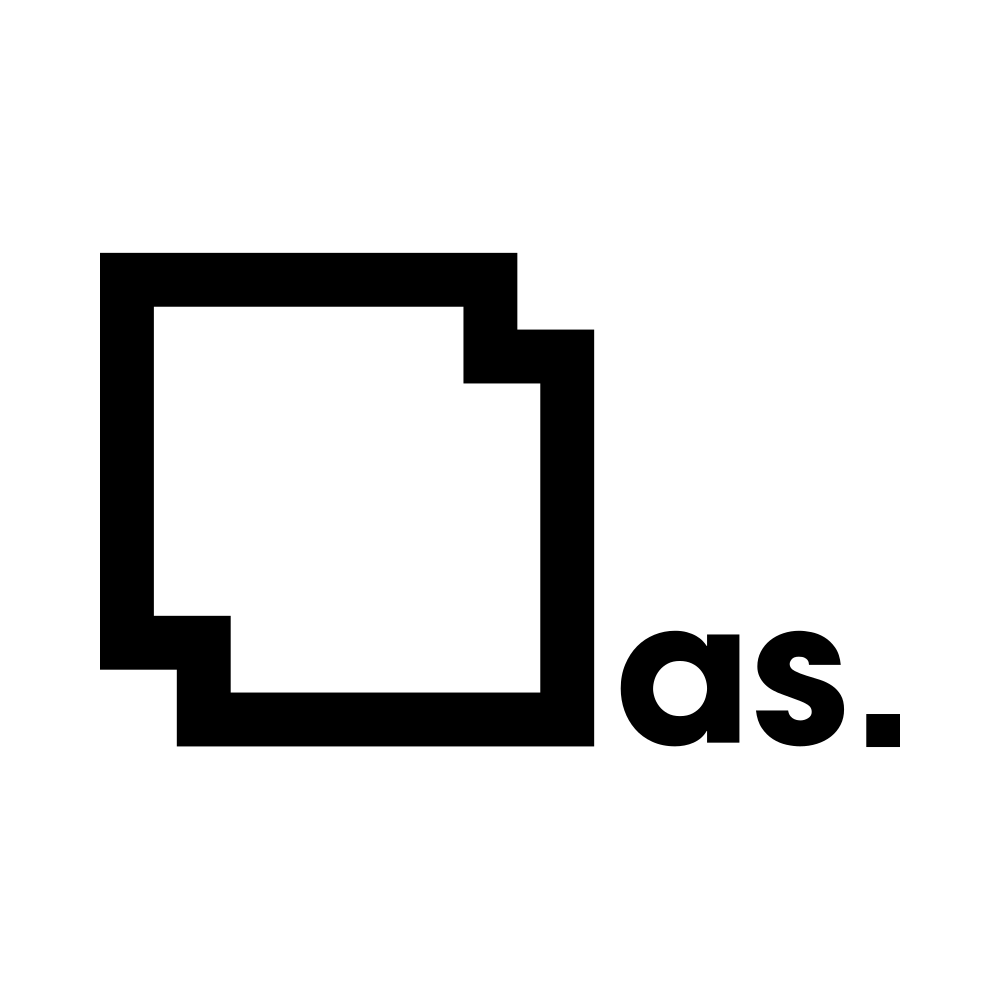
\includegraphics[height=6cm]{app_logo}
	\end{center}
	\caption {Logo di \acrlong{asd}.}
\end{figure}

Alternative Studio è una web agency che fornisce soluzioni professionali su misura, costruite secondo le esigenze del cliente. Si occupa
principalmente di sviluppo web e marketing. È un'azienda piccola che raccoglie poche risorse umane, ma molte energie che continuano a
spingere per crescere. Opera da appena sei anni nel settore del web development, ma ha abbracciato anche altre iniziative, collaborando in
progetti più grandi con altre realtà. Negli ultimi anni l'azienda si è cimentata nello sviluppo di un gestionale per l'organizzazione
\gls{ucis} e di una sua \acrshort{api} volta alla ricezione e all'elaborazione di attività registrate durante addestramento,
soccorso o esercitazioni.

%**************************************************************
\section{L'idea}

L'attuale applicazione per smartphone che si occupa di registrare le attività succitate è stata sviluppata molti anni fa ed essendo molto
instabile è nata l'esigenza di un refactoring di quest'ultima. Volendo utilizzare tecnologie moderne per lo sviluppo mobile e crossplatform
è nata l'esigenza di un'indagine preventiva sulle tecnologie da utilizzare. \\
Alternative Studio ha pensato, quindi, di aprire una posizione perfetta per un laureando, che cerchi un progetto formante, che lo metta continuamente alla prova.

%**************************************************************


\section{Strumenti utilizzati}

Lo stage si è focalizzato sull'utilizzo di tecnologie mobile per lo sviluppo di applicazioni per smartphone. Data la veloce evoluzione di
questo ramo, Alternative Studio ha avviato uno studio approfondito per scegliere quelle più adatte allo sviluppo della
propria applicazione. Di seguito alcune tecnologie che siamo andati a scegliere per lo sviluppo. Lo studio approfondito e le motivazioni
della scelta saranno spiegati in dettaglio nel \autoref{sec:studiodifattibilita}.

\subsection{Ionic}

Ionic è un \gls{framework} open source che fornisce strumenti agli sviluppatori, come librerie grafiche e plugins nativi per dialogare
con \gls{Android} e \gls{iOS}. Esso permette lo sviluppo mobile utilizzando tecnologie standard web come Angular, React e Vue, evitando lo
sviluppo in linguaggio nativo dei singoli sistemi operativi. Questo è reso possibili da wrapper esistenti su ogni piattaforma volti a
eseguire l'applicazione.

\subsection{Angular}

Come framework web per lo sviluppo \gls{frontend} si è utilizzato Angular, evoluzione del noto AngularJS, sviluppato in prevalenza da Google, ma con distribuzione \gls{open source}. Le applicazioni Angular sono eseguite direttamente lato client dal web browser e quindi non vengono reinviate indietro al web server. Inoltre sono nativamente responsive, cioè i toolkit utilizzate si adattano al dispositivo sul quale sono eseguite. \\
Nonostante l'esperenzia di Alternative Studio sull'analogo Vue, si è deciso di adottare Angular dato che Ionic-Vue era ancora in fase di
beta e quindi potenzialmente instabile e soggetto a cambiamenti.

\subsubsection{TypeScript}

TypeScript è un linguaggio implementato da Microsoft nel 2012, derivato da JavaScript, al quale aggiunge il concetto di tipizzazione e di orientamento agli oggetti. Nonostante JS sia un linguaggio \gls{tipizzato}, esso non fa nessun tipo di controllo statico sui tipi effettuando sempre una conversione dinamica. Questo produce spesso degli errori difficili da trovare e correggere, per questo TypeScript introduce la compilazione che non fa altro che tradurre il codice in JavaScript, eseguendo prima un controllo dei tipi.\\
Grazie a queste caratteristiche TypeScript non è stato utilizzato solo per il \gls{frontend}, ma anche per parte della logica
dell'applicazione. Per questo e per il fatto che è il linguaggio adottato nativamente da Angular sarà quello più utilizzato durante lo
sviluppo.

\subsection{Android e Java}

\gls{Android} è il sistema operativo mobile più diffuso nel pianeta e di proprietà di \gls{Google}. È stato scelto come riferimento durante
lo sviluppo, nonostante Ionic offra la possibilità di sviluppare in crossplatform con lo stesso codice. Al contrario alcune
funzionalità che si interfacciano con il sistema operativo, come ad esempio la componente GPS, devono essere sviluppate in linguaggio
nativo, che nel caso di \gls{Android} è \gls{java}.

%**************************************************************

\section{Metodo di Lavoro}
Dato le contenute risorse umane a disposizione Alternative Studio adotta un ciclo di sviluppo software \gls{Incrementale} con qualche
introduzione di processi da quello \gls{Agile}, in particolared dal metodo \gls{Scrum}. Durante lo stage lo studente è stato anche
incaricato di introdurre qualche concetto delle metodologie di sviluppo moderne all'interno del contesto aziendale, come quello di
\gls{Sprint} e di \gls{Daily Stand-up}.

\subsection{Processi di sviluppo}
La mia figura è subentrata durante la fase di Analisi dei requisiti. Per questo i primi compiti affidatomi sono stati quelli di studio delle
tecnologie adatte al progetto. Durante questa fase si sono svolte alcune riunioni con il tutor, tramite videochiamata,
e redatto alcuni documenti di report riguardo le ispezioni e le ricerche. Inoltre il lavoro individuale (come compilare un "Hello World" con Ionic) si è svolto
tramite tasks. Le riunioni con il tutor sono proseguite anche durante la fase di progettazione architetturale, durante la quale abbiamo
chiarito la visione generale dell'applicazione.

\subsection{Strumenti di supporto allo sviluppo}
Ci sono alcuni software da citare utilizzati nella gestione del progetto, che \acrlong{asd} utilizza abitualmente.

\subsubsection{Gestione progetto e Versione}
Gitlab è un software open source per la gestione di repository \gls{Git} e supporto alla Continous Integration.

\begin{figure}[htbp]
	\begin{center}
		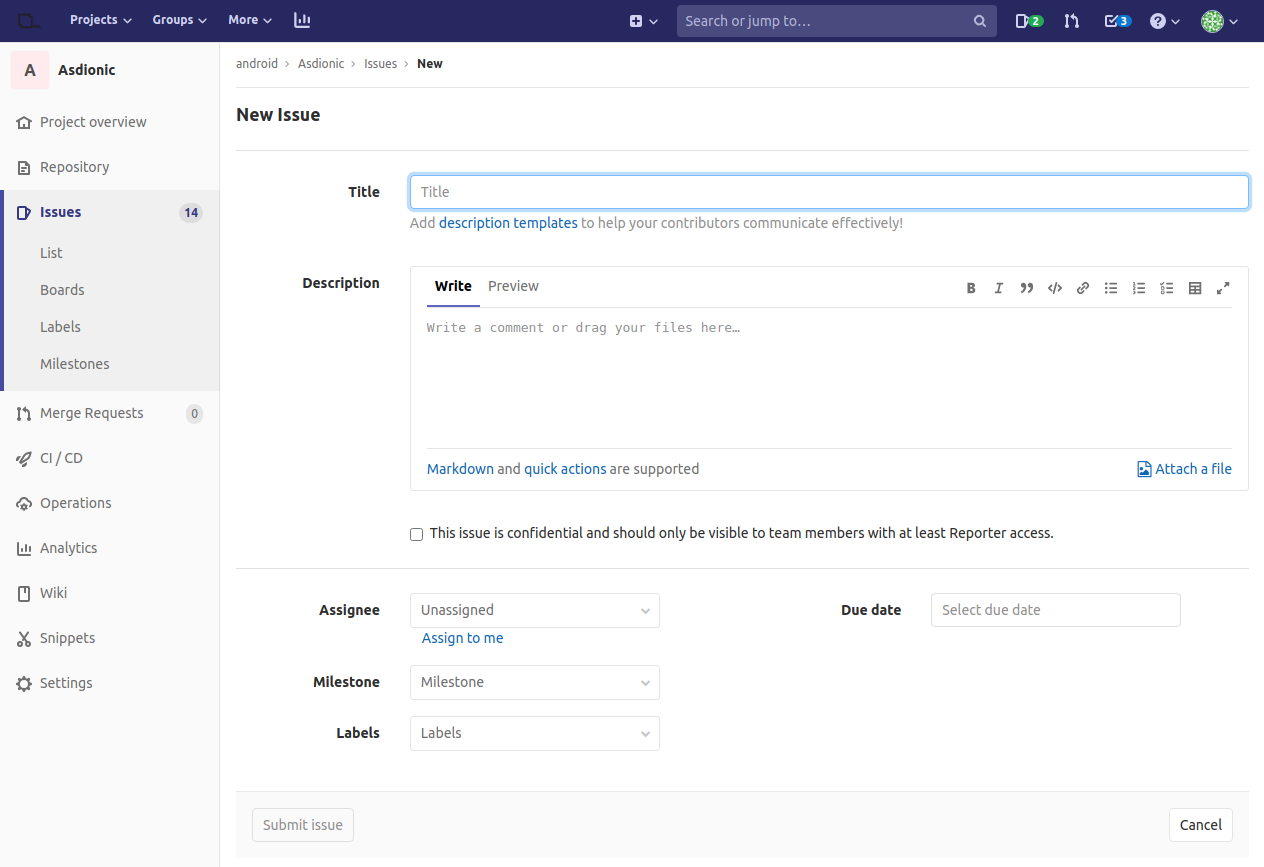
\includegraphics[height=8.5cm]{gitlab_schermata}
	\end{center}
	\caption {Schermata di nuova issue del software Gitlab.}
\end{figure}

\noindent Per la prima parte è stato importante il suo strumento di \gls{Issue Tracking System} con il quale si sono gestite le tasks e le
loro scadenze. Infatti, in questo caso le issues sono state utilizzate come metodo per tracciare i compiti da svolgere, piuttosto che per
segnalare problemi all'interno del software, come bug e affini. \\
\noindent Ogni task possiede un titolo significativo, una descrizione approfondita aggiornabile in caso di cambiamenti durante l'esecuzione
e una scadenza. Inoltre è possibile assegnarla a più membri del team, aggiungere informazioni o dialogare con il tutor attraverso la sezione
commenti e specificare la milestone alla quale è collegata.

\subsubsection{Comunicazione}
Causa il telelavoro, durante il progetto sono stati fondamentali gli strumenti di comunicazione:
\begin{itemize}
	\item Slack: per le comunicazioni ufficiali e come strumento di notifica per i cambiamenti nella repo.
	\item Telegram: come servizio di messaggistica istantanea, diretta con il tutor.
	\item Skype: per le videochiamate, essenziale per lo svolgersi delle riunioni a distanza.
\end{itemize}

\subsubsection{Codifica}
In dotazione ad Alternative Studio ho utilizzato WebStorm, potente IDE parte della suite di JetBrains. Una delle sue caratteristiche
principali sono la sua modularità, grazie allo store di plugins disponibili che aggiungono funzionalità, come il conteggio delle ore di
programmazione e gestione del repository \gls{Git} locale. \\
Inoltre si integra molto bene con le tecnologie web, come Angular, mettendo a disposizione il suo ambiente di building e di testing direttamente all'interno dell'\acrshort{ide}.

\begin{figure}[htbp]
	\begin{subfigure}{0.5\textwidth}
		
\includegraphics[height=2cm]{webstorm}
		\caption{Logo di WebStorm}
	\end{subfigure}
	\begin{subfigure}{0.5\textwidth}
		
\includegraphics[height=2cm]{studio}
		\caption{Logo di Android Studio}
	\end{subfigure}
\end{figure}

\subsubsection{Android Studio}
Android Studio fa parte sempre del pacchetto IDEA di JetBrains ed è una versione molto ridotta di Intellij. A differenza del suo
fratello maggiore è open source e ottimizzato per lo sviluppo Android. I linguaggi nativi utilizzabili in questo \acrshort{ide} sono principalmente
\gls{Go} e \gls{java}. Utilizza gradle come strumento automatico per la build dei progetti ed è estensibile come le altre applicazioni IDEA
tramite plugins.

\subsubsection{Postman}
Programma a supporto della codifica, il quale mi ha aiutato nell'interfacciarmi alle API. Postman permette di fare chiamate \acrshort{http} ad
un'API e di visualizzarne il risultato. È un software molto utile nel quale puoi, ad esempio, testare le stringhe che utilizzerai nel tuo
codice, o per analizzare il risultato per capire come utilizzarlo.
%**************************************************************
             % Introduzione
% !TEX encoding = UTF-8
% !TEX TS-program = pdflatex
% !TEX root = ../tesi.tex

%**************************************************************
\chapter{Descrizione dello Stage}
\label{cap:descrizione-stage}
%**************************************************************

% \intro{Brevissima introduzione al capitolo}

%**************************************************************
\section{Scelta dello Stage}

La scelta dello stage è stata molto difficile. Ero alla ricerca, infatti, di un contesto specifico per la mia prima esperienza lavorativa
nel settore informatico. Consultando tutte le varie proposte, durante l'evento Stage-IT, ho fatto fatica a trovare una proposta che mi
convincesse a fondo. Alcune delle aziende che ho contattato si sono dimostrate disponibili nei miei confronti, ma per tempistiche legate
alla laurea non siamo riusciti a venirci incontro.
%  Tra le motivazioni per le quali ho scelto \gls{asd} c'è senz'altro un progetto chiaro e
% stimolante, ma anche la disponibilità immediata allo stage.

\subsection{Motivazioni della scelta}

Quello di cui ero alla ricerca era un contesto piccolo con ampi margini di crescita e di formazione personale sulle tecnologie moderne, più
che sul metodo di lavoro, che invece tende a essere molto più definito in aziende grandi, con un modello affermato e utilizzato da tempo.
Quello che mi interessava era sperimentare vari ruoli, comprendere le varie responsabilità che questi comportano e come interfacciarsi con
altri dipendenti. \\
Oltre al contesto aziendale ero attratto anche dall'argomento del progetto. Volevo sperimentare nuove tecnologie e nuovi linguaggi,
disegnare e creare del software, piuttosto che mantenerlo o estenderlo. Da questo punto di vista l'Università di Padova,
attraverso Stage-IT mi ha messo in contatto con molte aziende interessanti. Inoltre la mia ricerca del progetto di stage si è basata sul desiderio
di lavorare in ambito frontend e questo ha ristretto di molto le varie opportunità. \\
Il fattore decisivo sulla scelta dello stage è stato il fatto che da tempo volevo sperimentare le tecnologie per lo sviluppo di applicazioni
mobile. Io stesso, precedentemente, avevo provato ad avviare qualche piccolo progetto in questo campo e per questo ho voluto
scegliere una proposta che avesse questo come tema principale. \\
In questo senso l'offerta di \acrlong{asd} ha subito catturato la mia attenzione e nonostante fosse la loro prima esperienza con uno
studente laureando, ho preso contatti per avviare con loro il mio stage.

\subsection{Obiettivi personali}
\label{sec:obiettivi-pers}
Le esperienze lavorative precedenti a questa mi avevano insegnato cosa vuol dire lavorare in una squadra e cos'è prendersi carico
di responsabilità, ma con nessuna di queste avevo messo in pratica ciò che avevo studiato finora. Sentivo quindi il bisogno di consolidare
il bagaglio di nozioni acquisite durante gli anni del corso e lo stage ne è stata l'occasione perfetta. Certo, ci sono stati i molteplici
progetti didattici, ma nulla è come entrare nel contesto lavorativo e avere contatto diretto con questa realtà. \\
Principalmente le mie aspirazioni si possono riassumere in:
\begin{itemize}
	\item collaborare con colleghi con molta più esperienza e conoscenza di me;
	\item imparare nuove tecnologie e distinguere quelle buone da quelle cattive;
	\item migliorare la mia gestione del tempo e organizzarmi con le scadenze dei vari compiti;
	\item trovare proposte e contatti per progetti futuri.
\end{itemize}

%**************************************************************

\section{La proposta di stage}

\acrlong{asd} ha aperto una posizione per uno stage a una persona interessata al mobile development, che potesse collaborare sia nella parte di analisi, che nella parte di codifica. Il progetto era incentrato sulla formazione sulle tecnologie mobile, per fare evolvere l'azienda anche su questo ramo cercando nuove opportunità.

\subsection{Il contesto}

Come già accennato {\hyperref[cap:introduzione]{nel primo capitolo}} Alternative Studio è un'azienda giovane che da 5 anni collabora con
\gls{ucis}. Durante questi anni è stato sviluppato un gestionale e un sito per la loro organizzazione.

% chiedere info sul gestionale

All'interno di questo gestionale è stata sviluppata un'\acrshort{api}, volta alla registrazione di log contenenti la posizione tramite
coordinate e alla creazione di una relativa traccia. A questo software attualmente si interfaccia un'applicazione sviluppata 5 anni fa, non
da \acrlong{asd}, e pubblicata nel 2018 con il nome di UCIS Report Tool. L'applicazione ha come funzionalità principale la creazione e la
gestione di attività, con la registrazione e l'invio di log contenenti la posizione del dispositivo sul quale esegue. Questa, però, non
risulta essere un prodotto professionale e utilizza tecnologie già vecchie e difficilmente manutenibili o aggiornabili. Inoltre sono stati
lamentati da \gls{ucis} alcuni bug e pochissima precisione nella registrazione della posizione. Dall'associazione nasce così l'esigenza di aggiornare
o riscrivere completamente l'applicazione. \\
\noindent Alternative Studio ha colto, quindi, l'opportunità di sviluppare una sua versione dell'applicativo e di proporlo poi all'organizzazione con la quale già collabora.

\subsection{Obiettivi dello stage}
\label{sec:obiettivi}

Durante la compilazione del Piano di Lavoro, documento che mette in chiaro ciò che andrà fatto durante lo stage, con il tutor sono stati fissati gli obiettivi principali dello stage, che qui sono elencati e raggruppati come obbligatori, desiderabili e facoltativi.

\begin{itemize}
	\item Obbligatori
	\begin{itemize}
		\item progettazione e realizzazione di applicazione mobile;
    \item implementare servizio di geolocalizzazione preciso nell’applicazione;
    \item versione beta da pubblicare sullo store.
	\end{itemize}

	\item Desiderabili
	\begin{itemize}
		\item applicazione cross-platform, combatibile anche su dispositivi datati;
    \item messa in produzione dell’applicazione.
	\end{itemize}

	\item Facoltativi
	\begin{itemize}
		\item implementazione delle notifiche push;
    \item integrazione di una chat;
    \item applicazione funzionante anche su dispositivi senza servizi Google.
	\end{itemize}
\end{itemize}

\subsection{Pianificazione}

In seguito si è discusso su come ripartire le ore e decidere quali processi mi avrebbero portato a soddisfare gli obiettivi sopra scritti.
Si è prodotta una pianificazione oraria che prevedeva gran parte della prima parte dello stage in formazione e creazione di una \gls{product
baseline} e una seconda parte di codifica e testing dell'applicazione, per chiudere con il collaudo e la pubblicazione sullo store Android.
\\
Il progetto di stage prevedeva circa 320 ore e in particolare si era stimata la durata delle varie attività:
\begin{itemize}
		\item \textbf{Prima Settimana}
		\begin{itemize}
				\item Analisi e formazione delle tecnologie da utilizzare nel progetto;
				\item studio del framework ionic;
				\item studio di geolocalizzazione;
				\item studio per notifiche push.
		\end{itemize}
		\item \textbf{Seconda Settimana}
		\begin{itemize}
			\item Prototipo applicazione funzionante;
			\item implementazione funzionalità di gestione delle utenze;
			\item navigazione tra schermate dell’app.
		\end{itemize}
		\item \textbf{Terza Settimana}
		\begin{itemize}
				\item implementazione registrazione delle attività.
		\end{itemize}
		\item \textbf{Quarta Settimana}
		\begin{itemize}
				\item implementazione del salvataggio offline dei dati.
		\end{itemize}
		\item \textbf{Quinta Settimana}
		\begin{itemize}
				\item aggiunta chiamante API al gestionale.
		\end{itemize}
		\item \textbf{Sesta Settimana}
		\begin{itemize}
				\item implentazione gestione emergenze.
				\item test.
		\end{itemize}
		\item \textbf{Settima Settimana}
		\begin{itemize}
				\item collaudo;
				\item messa in produzione.
		\end{itemize}
		\item \textbf{Ottava Settimana}
		\begin{itemize}
				\item aggiunta requisiti facoltativi.
		\end{itemize}
\end{itemize}

I dettagli sono riportati sul seguente \gls{diagramma di Gantt}.

\begin{figure}[h]
	\begin{center}
		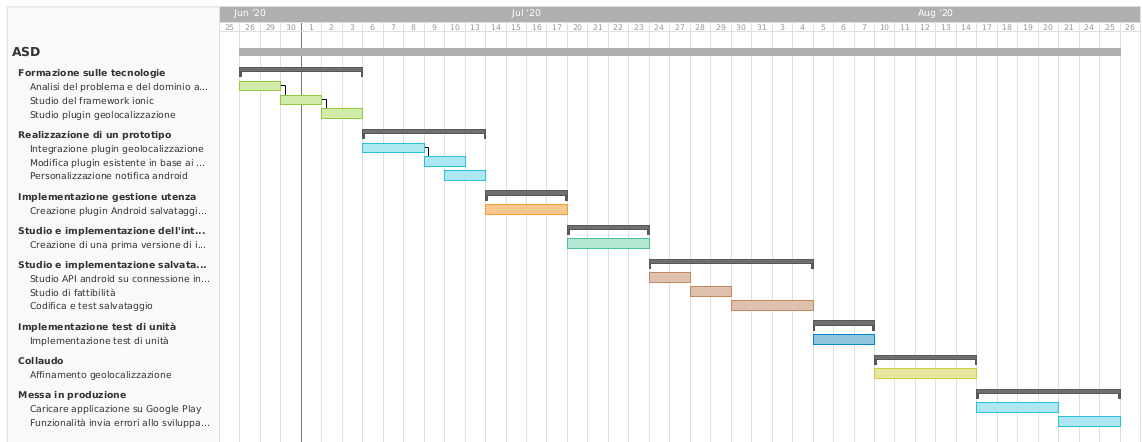
\includegraphics[height=6cm]{gantt}
		\caption{\Gls{diagramma di Gantt} della ripartizione giornaliera.}
	\end{center}
\end{figure}

\subsection{Vincoli}

Questo capitolo si occupa di descrivere i vincoli ai quali sono stato sottoposto durante lo stage. Tengo a precisare che quelli imposti dall'azienda non sono mai stati un ostacolo, bensì delle guide precise per raggiungere al meglio gli obiettivi. I vincoli sono stati raggruppati nelle sezioni successive.

\subsubsection{Vincoli tecnologici}
Il vincolo più importante imposto è stato quello di non scrivere l'applicazione in linguaggio nativo per ogni sistema operativo. Nonostante
sia stata sviluppata solamente per il sistema operativo Android, l'idea iniziale era quella di produrla \gls{crossplatform} e di portarla con
poche modiche su qualunque sistema operativo mobile e non. È per questo che il tutor mi ha imposto la ricerca di un framework ibrido.

\subsubsection{Vincoli metodologici}
Il mio stage si è svolto, purtropp o, durante un periodo soggetto a restrizioni negli spostamenti dovuti all'epidemia di SARS-CoV-2. Dopo un
periodo iniziale, però, sono riuscito a svolgere lo stage in parte in presenza. Quinid ho concordato con il tutor di poter accedere ai locali di
Alternative Studio almeno due giorni a settimana, solitamente il lunedì e il venerdì. \\
Per quanto riguarda il metodo di lavoro ho cercato diverse volte consiglio presso il tutor. Riuscire a svolgere lo stage in presenza, anche
se in parte, è stato molto importante in questo senso. Infine per aderire in parte al metodo \gls{Agile} abbiamo organizzato una breve riunione
giornaliera, che aveva come scopo quello di allineare il lavoro e programmare le tasks successive.

\subsubsection{Vincoli temporali}
Oltre al vincolo di 320 ore, imposto dalla natura dello stage e dall'azienda stessa, sono dovuto sottostare alle scadenze delle varie tasks
impostate su Gitlab. In particolare si è scelto di lavorare 40 ore alla settimana. \\
Non essendo stato  uno stage completamente in presenza, non si è dato nessun vincolo sulla singola giornata lavorativa. Solitamente l'orario
lavorativo iniziava alle 9:00 e si concludeva alle 18, con un'ora di pausa pranzo. Questo per me è stato un problema da affrontare, perché
ho notato che sono molto più produttivo quando ho delle restrizioni sugli orari. Il problema è stato fatto presente al tutor che ha
collaborato nel controllo e nel conteggio delle ore effettiva di lavoro.
             % Processi
% !TEX encoding = UTF-8
% !TEX TS-program = pdflatex
% !TEX root = ../tesi.tex

%**************************************************************
\chapter{Descrizione dello stage}
\label{cap:descrizione-stage}
%**************************************************************

\intro{Breve introduzione al capitolo}

%**************************************************************
\section{Introduzione al progetto}

%**************************************************************
\section{Analisi preventiva dei rischi}

Durante la fase di analisi iniziale sono stati individuati alcuni possibili rischi a cui si potrà andare incontro. Si è quindi proceduto a elaborare delle possibili soluzioni per far fronte a tali rischi.
\begin{risk}{Performance del simulatore hardware}
    \riskdescription{le performance del simulatore hardware e la comunicazione con questo potrebbero risultare lenti o non abbastanza buoni da causare il fallimento dei test}
    \risksolution{coinvolgimento del responsabile a capo del progetto relativo il simulatore hardware}
    \label{risk:hardware-simulator}
\end{risk}

%**************************************************************
\section{Requisiti e obiettivi}


%**************************************************************
\section{Pianificazione}
             % Kick-Off
% !TEX encoding = UTF-8
% !TEX TS-program = pdflatex
% !TEX root = ../tesi.tex

%**************************************************************
\chapter{Valutazione Retrospettiva}
\label{cap:valutazione-retrospettiva}
%**************************************************************

% \intro{Breve introduzione al capitolo}

\section{Obiettivi raggiunti}
\subsection{Obiettivi dello stage}
In questa sezione analizzerò quali degli obiettivi descritti nel \hyperref[sec:obiettivi]{capitolo 2} sono stati raggiunti e quali no, dando
una giustificazione nel caso negativo.

\renewcommand{\arraystretch}{2}
\begin{longtable}{|p{10cm}|p{4cm}|}%
  \caption{Tabella degli obiettivi} 
  \label{tab:obiettivi} \\
    \hline
    \textbf{Obiettivo} & \textbf{Risultato} \\
    \hline
    \endhead
    \multicolumn{2}{|l|}{\textbf{Obbligatori}} \\ \hline
    Progettazione e realizzazione di applicazione mobile                      & Soddisfatto \\ \hline
    Implementazione servizio di geolocalizzazione preciso nell’applicazione   & Soddisfatto \\ \hline
    Versione beta dell'applicazione da pubblicare sullo store                 & Soddisfatto \\ \hline
    \multicolumn{2}{|l|}{\textbf{Desiderabili}} \\ \hline
    Applicazione cross-platform, combatibile anche su dispositivi datati      & Soddisfatto \\ \hline
    Messa in produzione dell’applicazione                                     & Soddisfatto \\ \hline
    \multicolumn{2}{|l|}{\textbf{Facoltativi}} \\ \hline
    Implementazione delle notifiche push                                      & Non Soddisfatto \\ \hline
    Integrazione di una chat                                                  & Non Soddisfatto \\ \hline
    Applicazione funzionante anche su dispositivi senza servizi Google        & Non Soddisfatto \\ \hline
\end{longtable}%

\noindent In generale sono stati rispettati tutti gli obiettivi, tranne quelli ritenuti facoltativi. Questi non erano inseriti nel piano di lavoro, se
non nell'ultima settimana in caso l'applicazione fosse stata già pronta. In ogni caso gli obiettivi facoltativi inseriti fanno parte dei requisiti
dell'applicazione e per questo non sono stati esclusi completamente. Durante lo stage ho infatti studiato i metodi per le notifiche push su
\gls{Android} e su come sviluppare applicazioni in dispositivi senza servizi Google, come ad esempio alcuni modelli recenti \textit{Huawei}.
\\
\noindent Grazie al metodo di lavoro utilizzato, ho rispettato anche il piano di lavoro concordato con il tutor aziendale. Le brevi riunioni quasi
giornaliere durante le quali si definivano le piccole task, sono state molto utili allo scopo, velocizzando lo sviluppo e razionalizzando il
tempo a disposizione per ognuna di esse. 

\subsection{Obiettivi personali}
Questo stage aveva anche alcuni obiettivi personali descritti nella sezione \hyperref[sec:obiettivi-pers]{2.1.2}:
\begin{itemize}
    \item Alternative Studio mi ha dato la possibilità di collaborare a stretto contatto con professionisti nel settore che mi hanno formato
    e hanno plasmato il mio metodo di lavoro. Sono stato contento di aver lavorato in un contesto giovane e in espansione, dove un giovane
    stagista può sentirsi a proprio agio crescendo assieme alla realtà in cui è immerso. Nonostante questo mi sento di aver imparato a
    distinguere ciò che è \textit{professionale} da ciò che non lo è.
    \item Nella sezione successiva descriverò in dettaglio quali tecnologie ho imparato. In generale penso che la lunga analisi avviata
    nello studio di fattibilità mi abbia aiutato e fatto capire cosa mi propone il mondo informatico. Sono riuscito a sviluppare un metodo
    per esaminare e sviscerare le caratteristiche di ognuna delle tecnologie, che consiste nelle leggere la documentazione ufficiale,
    costruire una mia opinione e solo in seguito leggere opinioni di altri, cercando ovviamente le più autorevoli. Ho capito anche che un
    buon software non è composto solo da una buona codifica, una buona interfaccia o un buon supporto, ma da una grande community che
    fornisce un troubleshooting adeguato a tutti i problemi che puoi incorrere.
    \item Sono abbastanza soddisfatto di come sia riuscito a gestire il tempo. Ero molto preoccupato che la gestione elastica dettata dal
    telelavoro mi avrebbe penalizzato, date le distrazioni "casalinghe", o al contrario non avere orari di ufficio mi avrebbe portato a fare
    più ore di quelle stabilite. Non nascondo che è ovviamente capitato, quando uno sviluppatore si intestardisce nel trovare una
    soluzione a un problema può rimane anche ore su di esso, ma spesso il tutor è intervenuto a regolarizzare il ritmo lavorativo. 
    \item Grazie a Stage-IT sono riuscito a raccogliere molti contatti. Mi piacerebbe continuare a collaborare con \acrlong{asd} nei suo
    progetti futuri.
\end{itemize}

\section{Conoscenze e competenze acquisite}
\subsection{Collaborazione con i colleghi}
Il lavoro di squadra era uno dei punti che più mi preoccupava. Prima dello stage ero convinto che iniziare un progetto in più persone senza
dividere bene i ruoli e le mansioni in modo definito fosse impossibile. Dopo questa esperienza mi sento di dire che lavorare in un team
cercando il confronto continuo e avendo sempre qualcuno a supporto è il modo migliore per raggiungere gli obiettivi. \\ 
\noindent Ho capito che il fallimento è contemplato in questo settore e che se una cosa non riesce puoi sempre rivolgerti a qualcun altro
che ti darà una visione diversa del problema. Questo approccio mi è tornato utile molto spesso durante il progetto quando mi trovavo fermo
in punto, senza trovare vie d'uscita, rivolgermi al tutor è sempre stata la soluzione migliore.
\noindent Un'altro aspetto al quale tengo molto e la gestione delle relazioni tra colleghi che deve andare oltre al semplice rapporto
lavorativo, per creare un ambiente rilassato e confortevole, dove è più semplice lavorare. Ho imparato quindi a essere professionale, ma al
contempo non troppo rigido.

\subsection{Analisi e Studio di Fattibilità}
Prima di intraprendere il percorso di stage la consideravo una fase noiosa e poco utile di un progetto. Ho completamente cambiato idea
affrontandola con il tutor. In precedenza, probabilmente avevo un approccio meno interattivo e un po' retrogrado, ma con il tutor sono
riuscito a cambiarlo radicalmente. \\ 
\noindent Dato che i requisiti erano già stati quasi tutti fissati, lo studio delle tecnologie da utilizzare è quello che mi ha coinvolto di
più. Capire le caratteristiche di ognuna di esse e apprezzarne le differenze mi ha appassionato portandomi ad apprezzare questo processo
che prima ritenevo superfluo. È da sottolineare che questo progetto partendo da zero, aveva bisogno di un analisi completa e questo mi ha
dato molta libertà nella ricerca. 

\subsection{Tecnologie apprese}
Oltre ad affinare l'utilizzo di Git e degli strumenti di controllo di versione, ho appreso meglio il concetto di \gls{ci}
attraverso gli strumenti di GitLab. Ho conosciuto il mondo dello sviluppo mobile e di tutte le tecnologie che ci stanno attorno, ordinando
le conoscenze acquisite in precedenza. È stato affascinante passare da utente di applicazioni per smartphone a programmatore, iniziando a
notare tutti gli stessi errori e le imperfezioni che altri sviluppatori hanno commesso come me su alcune cose. \\
\noindent Ho imparato a programmare con Ionic e Angular, che sicuramente mi saranno utili in futuro nel mondo del web development. Ora sono
in grado di gestire in modo efficiente la programmazione concorrente attraverso le librerie di \gls{nodejs} con le \textit{Promise}. So
interfacciarmi con delle API su un server web. Ho imparato, inoltre, a avviare un progetto in Android tramite il framework nativo e
modificare le sue parti in \acrshort{xml} e \gls{java}.

\section{Valutazioni personali}
Ritengo di aver avuto parecchie aspettative sullo stage finale, considerandolo la conclusione di un percorso che mi avrebbe lanciato poi nel
mondo del lavoro e testando tutte le mie conoscenze apprese durante gli studi. Ho scoperto però che non è stato del tutto così. Avrei dovuto
affrontarlo con aspettative più basse e un altro tipo di mentalità. Non è stata un'esperienza negativa, al contrario ho imparato molto e
credo sia quella più utile proposta dal corso di laurea, ma da questa ho scoperto che mi mancano ancora moltissime competenze e conoscenze
per essere del tutto pronto al mondo del lavoro. \\
\noindent Nel complesso mi sento soddisfatto e credo di aver fatto un ottimo lavoro, mettendo tutto me stesso nel progetto e impegnandomi
nella sua realizzazione. Grazie al contesto aziendale nel quale mi sono trovato ho avuto tutti gli strumenti per crescere e spero di
trovarne di simili nel prossimo futuro. So che dovrò spendere molto più delle 300 ore messe a disposizione dallo stage per sentirmi
completamente realizzato e pronto per diventare un vero e proprio informatico.             % Concept Preview

%**************************************************************
% Materiale finale
%**************************************************************
\backmatter

\glsaddall

\printglossary[type=\acronymtype]

\printglossary

% !TEX encoding = UTF-8
% !TEX TS-program = pdflatex
% !TEX root = ../tesi.tex

%**************************************************************
% Bibliografia
%**************************************************************

\cleardoublepage
\chapter{Bibliografia}

\nocite{*}
% Stampa i riferimenti bibliografici
% \printbibliography[heading=subbibliography,title={Riferimenti bibliografici},type=book]
% \printbibliography[heading=subbibliography,title={Riferimenti bibliografici}]

% Stampa i siti web consultati
% \printbibliography[heading=subbibliography,title={Siti web consultati},type=online]
\printbibliography[heading=subbibliography,title={Siti web consultati}]


\end{document}
